\documentclass[10pt,a4paper]{article}
\usepackage[margin=0.82in]{geometry}
\usepackage[T1]{fontenc}
\usepackage{lmodern,microtype,booktabs,graphicx,xcolor,hyperref}
\hypersetup{hidelinks}
\setlength{\parindent}{0pt}\setlength{\parskip}{6pt}
\title{IDM-Viz: Exact-Interval Sensitivity on UCI 224}
\author{Ahmed Bilal (23I-2581) \and Umar Behram (23I-2604)}
\date{16 November 2026}
\begin{document}\maketitle
\begin{abstract}
We recomputed the existing UCI 224 plug-in correctness intervals using the exact Poisson-binomial distribution and compared them with the original continuity-corrected normal approximation on identical cached predictions. Exact intervals covered 0 of 9 monitoring cohorts, the same count as the normal approximation. Their mean width was 0.0234, versus 0.0258. Thus normal approximation error does not explain the external calibration failure.
\end{abstract}
\section{Design}
This post-hoc sensitivity extension used frozen probabilities from the existing single-model UCI 224 cohort study. No model or calibrator was refit and no cohort outcome was used to select a method. For cohort $b$, the exact calculation forms the distribution of $S_b=\sum_i Z_i$ with independent $Z_i\sim\mathrm{Bernoulli}(q_i)$, then reports discrete 2.5\% and 97.5\% quantiles of $S_b/n_b$. The comparator recomputes the original normal approximation with continuity correction from the same $q_i$. The nine sequential cohorts are descriptive, not independent replications.
\section{Results}
The mean absolute error of the calibrated accuracy point estimate remained 0.545. Exact intervals were narrower by 0.0024 on average; mean absolute endpoint displacement was 0.0013. Both approaches covered 0/9 realized cohort accuracies. The substantial gap between estimated and realized accuracy is therefore not fixed by replacing the approximation algorithm.
\begin{figure}[ht]\centering
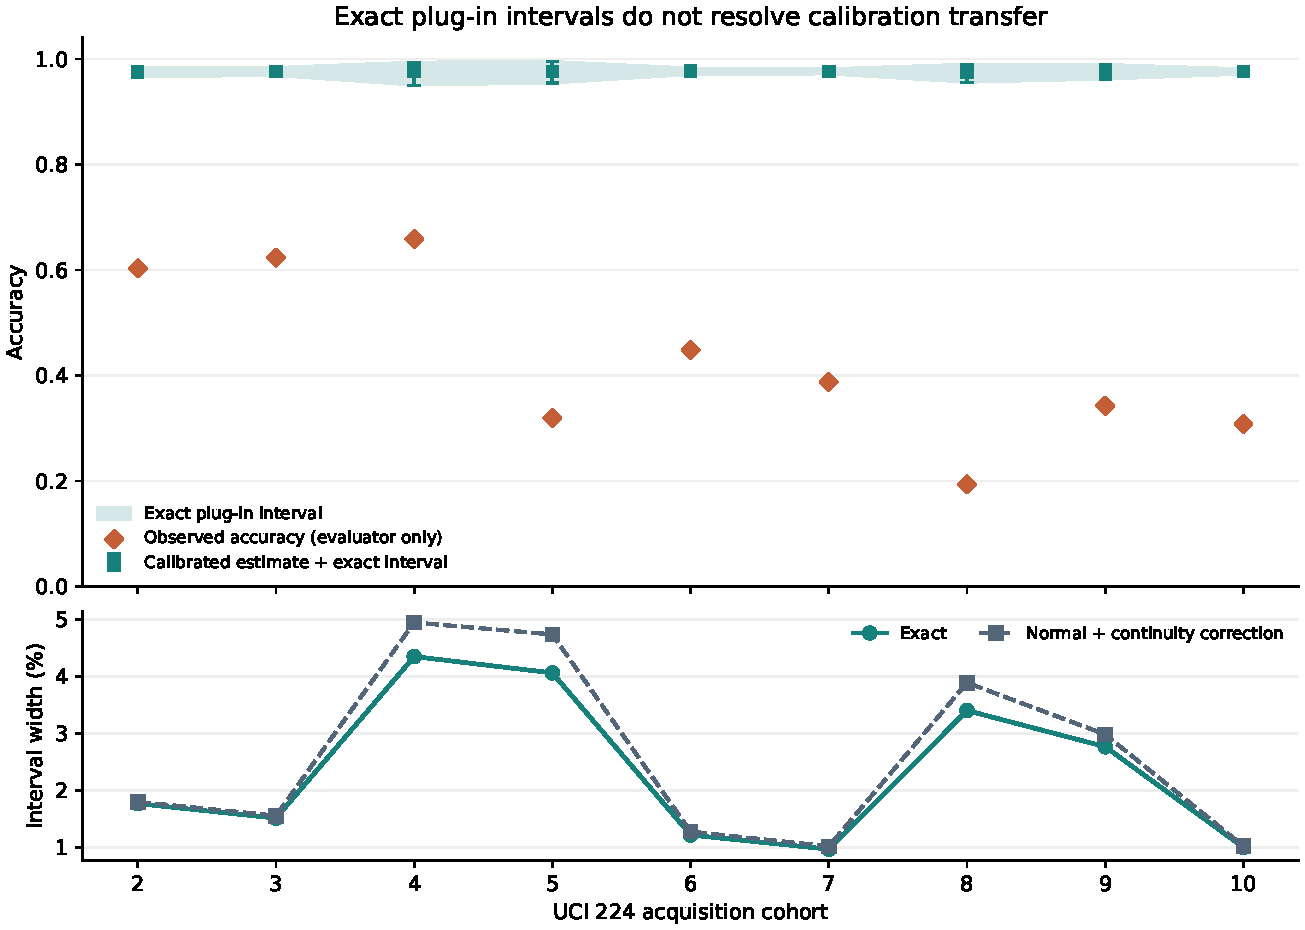
\includegraphics[width=0.93\linewidth]{interval_comparison.pdf}
\caption{Observed cohort accuracy compared with the fixed calibrated correctness estimate and its exact plug-in interval (top); exact and normal-approximation interval widths (bottom). Outcomes are shown for retrospective evaluation, never as online inputs.}
\end{figure}
\section{Interpretation and limits}
The exact calculation is numerically preferable for this finite Poisson-binomial model, but it does not repair a correctness model that transfers poorly across cohorts. Both intervals condition on fitted $q_i$ values, assume independent correctness indicators, omit calibration and reference uncertainty, and lack arbitrary-shift coverage guarantees. The one UCI dataset and its acquisition cohorts do not establish domain generality. This analysis is exploratory and does not supersede the original external result.
\section{Reproduction}
\begin{verbatim}
python scripts/evaluate_uci224_exact_interval_extension.py \\
  --out results/phase3/external_uci224_exact_interval_NEW
python scripts/report_uci224_exact_interval_extension.py
\end{verbatim}
The original Phase 2 DOCX and earlier reports are unchanged.\end{document}
